\documentclass[12pt,titlepage,openright,twoside]{report}
\usepackage[a5paper,showframe]{geometry}
\usepackage[notlot]{tocbibind} % for having bibliography, list of figures, etc.. in the table of contents (nottoc,notlof,notlof for not displaying toc, lof, lot)
\usepackage[italian]{babel}
\usepackage[utf8]{inputenc}
\usepackage{fontenc}
\usepackage{url} % per gestione url nella bibliografia
\usepackage{amsmath} % per tutte le formulacce matematiche
\usepackage{mathdots} 
\usepackage{amssymb} % per r reali
\usepackage{amscd} % per diagrammi
\usepackage{caption}
\usepackage{subcaption}
\usepackage{graphicx} % per immagini
\usepackage[margin=10pt,font=small,labelfont=bf,labelsep=endash]{caption} % didascalie personalizzate
\usepackage{fancyhdr}%per intestazione personalizzata
\usepackage[bookmarks,hidelinks]{hyperref} % for pdf index and links
\usepackage{enumerate} % for small roman letters in enumerate
\usepackage{algorithm} % for algorithms
\usepackage{algpseudocode}
\usepackage[acronyms,nopostdot,nogroupskip,toc,nonumberlist]{glossaries}
\usepackage{booktabs}
\usepackage{tabularx}
\usepackage{cite} % for citation grouping
\usepackage{pdfpages}

\setlength{\headheight}{15pt}
%Comandi per apici e peidici in text
\newcommand{\pedic}[2]{#1_{\text{#2}}}
\newcommand{\apic}[2]{#1^{\text{#2}}}
\newcommand{\apicpedic}[3]{#1^{\text{#2}}_{\text{#3}}}
\newcommand{\modulus}[1]{\left| #1 \right|}
\newcommand{\boldText}[1]{\text{\textbf{#1}}}

\renewcommand{\arraystretch}{1.4}
\renewcommand{\alglinenumber}[1]{\tiny#1:}

\newcolumntype{b}{X}
\newcolumntype{s}{>{\hsize=.5\hsize}X}
\newcolumntype{a}{>{\hsize=.4\hsize}X}
\newcolumntype{r}{>{\hsize=.2\hsize}X}

\makeatletter
\newcounter{imagepage}
\newcommand*{\foreachpage}[2]{%
  \begingroup
    \sbox0{\includegraphics{#1}}%
    \xdef\foreachpage@num{\the\pdflastximagepages}%
  \endgroup
  \setcounter{imagepage}{0}%
  \@whilenum\value{imagepage}<\foreachpage@num\do{%
    \stepcounter{imagepage}%
    #2\relax
  }%
}
\makeatother


%%========================================================
%%     modifica dimensioni layout larghezza pagina
%%
\addtolength{\textwidth}{7mm}%aumento larghezza testo
\addtolength{\hoffset}{-3.5mm}%diminuisco colonna per note a fianco per centrare testo allargato
\addtolength{\evensidemargin}{-1mm}%sposto la colonna di testo delle pagine pari a sinistra
\addtolength{\oddsidemargin}{1mm}%sposto la colonna di testo delle pagine dispari a destra
%%
%%========================================================

%%========================================================
%%            personalizzazione intestazione
%%
% i comandi seguenti impediscono la scrittura in maiuscolo
% dei nomi dei capitoli e dei paragrafi nelle intestazioni
\renewcommand{\chaptermark}[1]{\markboth{#1}{}}
\renewcommand{\sectionmark}[1]{\markright{\thesection\ #1}}
\fancyhf{} % rimuove l’attuale contenuto dell’intestazione
            % e del pi\‘e di pagina
%opzioni da mettere per twoside
\fancyhead[LE,RO]{\thepage}
\fancyhead[LO]{\nouppercase\rightmark}%\nouppercase elimina tutte le intestazioni maiuscole
\fancyhead[RE]{\nouppercase\leftmark}%\nouppercase elimina tutte le intestazioni maiuscole
%
%opzioni da mettere per oneside
%\fancyhead[RO]{\thepage}
%\fancyhead[LO]{\rightmark}
%
\renewcommand{\headrulewidth}{0.5pt}
\renewcommand{\footrulewidth}{0pt}
\addtolength{\headheight}{1.7pt} % riserva spazio per la linea
\fancypagestyle{plain}{%ridefinisce lo stile plain usato nelle pagine di chapter
\fancyhead{} % ignora, nello stile plain, le intestazioni
   \renewcommand{\headrulewidth}{0pt} % e la linea
   \fancyfoot[C]{\thepage}%per avere numero pagina anche pagina iniziale chapter
}
%%
%%========================================================

%%========================================================
%%   per imporre sillabazione
%%
\hyphenation{STSK}%
%%========================================================

%%========================================================
%%   list of acronyms
%%
%%\loadglsentries{sources/acronyms.tex}
\newacronym{doa}{DOA}{direction of arrival}
\newacronym{gnss}{GNSS}{Global Navigation Satellite System}
\newacronym{bs}{BS}{base station}
\newacronym{ms}{MS}{mobile station}
\newacronym{tof}{TOF}{time of flight}
\newacronym{toa}{TOA}{time of arrival}
\newacronym{tdoa}{TDOA}{time difference of arrival}
\newacronym{3gpp}{3GPP}{Third Generation Partnership Project}
\newacronym{lte}{LTE}{Long-Term Evolution}
\newacronym{4g}{4G}{fourth generation}
\newacronym{fdd}{FDD}{Frequency Division Duplexing}
\newacronym{re}{RE}{Resource Element}
\newacronym{rb}{RB}{Resource Block}
\newacronym{pss}{PSS}{Primary Synchronization Signal}
\newacronym{sss}{SSS}{Secondary Synchronization Signal}
\newacronym{pbch}{PBCH}{Physical Broadcast Channel}
\newacronym{cir}{CIR}{Channel Impulse Response}
\newacronym{cfr}{CFR}{Channel Frequency Response}
\newacronym{rss}{RSS}{received signal strength}
\newacronym{emw}{EMW}{electromagnetic waves}
\newacronym{gps}{GPS}{Global Positioning System}
\newacronym{agps}{A-GPS}{Assisted GPS}
\newacronym{glonass}{GLONASS}{Globalnaya Navigatsionnaya Sputnikovaya Sistema}
\newacronym{los}{LOS}{Line of Sight}
\newacronym{meo}{MEO}{medium Earth orbit}
\newacronym{ofdm}{OFDM}{Orthogonal Frequency Division Multiplexing}
\newacronym{ofdma}{OFDMA}{Orthogonal Frequency Division Multiple Access}
\newacronym{gsm}{GSM}{Global System for Mobile Communications}
\newacronym{umts}{UMTS}{Universal Mobile Telecommunications System}
\newacronym{prs}{PRS}{Positioning Reference Signal}
\newacronym{crs}{CRS}{Cell Specific Reference Signal}
\newacronym{rf}{RF}{radio frequency}
\newacronym{fft}{FFT}{Fast Fourier Transform}
\newacronym{ifft}{IFFT}{Inverse Fast Fourier Transform}
\newacronym{dft}{DFT}{Discrete Fourier Transform}
\newacronym{idft}{IDFT}{Inverse Discrete Fourier Transform}
\newacronym{isi}{ISI}{ InterSymbol Interference}
\newacronym{cp}{CP}{Cyclic Prefix}
\newacronym{ps}{PS}{Parallel to Serial}
\newacronym{hsr}{HSR}{Hochschule F\"{u}r Technik Rapperswil}
\newacronym{qam}{QAM}{Quadrature amplitude modulation}
\newacronym{psk}{PSK}{Phase-shift keying}
\newacronym{dac}{DAC}{Digital to Analog Conversion}
\newacronym{adc}{ADC}{Analog to Digital Conversion}
\newacronym{sra}{SRA}{Super Resolution Algorithm}
\newacronym{fcm}{FCM}{Forward correlation matrix}
\newacronym{fbcm}{FBCM}{Forward-backward correlation matrix}
\newacronym{music}{MUSIC}{multiple signals classification}
\newacronym{ev}{MUSIC eigenvalue}{EV}
\newacronym{esprit}{ESPRIT}{estimation of signal parameters via rotational invariance techniques}
\newacronym{dt}{DT}{discrete time}
\newacronym{svd}{SVD}{singular value decomposition}
\newacronym{ls}{LS}{least squares}
\newacronym{tls}{TLS}{total least squares}
\newacronym{mdl}{MDL}{minimum descriptive length}
\newacronym{iid}{IID}{independent and identically distributed}
\newacronym{snr}{SNR}{signal-to-noise ratio}
\newacronym{dlr}{DLR}{Deutschen Zentrums f\"{u}r Luft- und Raumfahrt}
\newacronym{lbs}{LBS}{location-based services}
\newacronym{awgn}{AWGN}{additive White Gaussian noise}
%%========================================================

%%========================================================
%%   comandi personalizzati
%%
\newcommand\numberthis{\addtocounter{equation}{1}\tag{\theequation}}
\newcommand{\realpin}[1]{\mathbb{R}\text{e}\{ #1 \}}
\newcommand{\imagpin}[1]{\mathbb{I}\text{m}\{ #1 \}}
\newcommand{\realp}[1]{\mathbb{R}\text{e}\left \{ #1 \right \}}
\newcommand{\imagp}[1]{\mathbb{I}\text{m}\left \{ #1 \right \}}
\newcommand{\phasein}[1]{\text{arg}\{ #1 \}}
\newcommand{\phase}[1]{\text{arg}\left \{ #1 \right \}}
\newcommand{\fcar}{f_\text{c}}
\newcommand{\fdop}{f_\text{D}}
\newcommand{\fdopn}{f_{\text{D},n}}
\newcommand{\fdopnm}{f_{\text{D},n,m}}
\newcommand{\average}[1]{\mathbb{E} \left[ #1 \right] }
\newcommand{\averagein}[1]{\mathbb{E} [ #1 ]}
\newcommand{\tra}{\text{T}}
\newcommand{\her}{\text{H}}
\newcommand{\vecop}[1]{\text{vec}\left( #1 \right)}
\newcommand{\vecopin}[1]{\text{vec}( #1 )}
\newcommand{\variance}[1]{\text{Var}\left( #1 \right)}
\newcommand{\variancein}[1]{\text{Var}( #1 )}
\newcommand{\tr}[1]{\text{tr} \left( #1 \right)}
\newcommand{\rank}[1]{\text{rank} ( #1 )}
\newcommand{\trin}[1]{\text{tr}( #1 )}
\newcommand{\bpsonhz}{\left[  \frac{\text{bps}}{\text{Hz}} \right]}
\newcommand{\bpsonhzin}{[ \frac{ \text{bps} }{ \text{Hz} } ]}
%%========================================================

%\linespread{1.2}

\allowdisplaybreaks[1] % Per spezzare equazioni su più righe
\makenoidxglossaries

\begin{document}
\raggedbottom % Prevent vertical justification
%%========================================================
%%  italian abstract and acknowledgements
\pagenumbering{roman}
%\thispagestyle{empty}
\vspace*{15ex}
\begin{flushright}
\textit{La Fede e la Ragione sono come le due ali \\
con le quali lo spirito umano s'innalza \\
verso la contemplazione della verit\`a.\\}
\vspace{4ex}
\scriptsize{San Giovanni Paolo II.}
\end{flushright}
\cleardoublepage

\chapter*{Abstract}
\label{chap:abstract}
\addcontentsline{toc}{chapter}{Abstract}
Negli ultimi anni, la grande crescita tecnologica dei sistemi wireless ha permesso lo sviluppo di nuovi
servizi ed applicazioni, disponibili in qualunque luogo per mezzo dei dispositivi mobili.
Molti di questi servizi, possono operare al meglio solo conoscendo la posizione del dispositivo.
Per questo motivo, i servizi basati sul posizionamento (LBS) hanno riscontrato negli ultimi anni un 
grande interesse, richiedendo ai moderni sistemi wireless, l'implementazione di sistemi di posizionamento
integrati nel dispositivo. 
%\chapter*{Acknowledgements}
\label{chap:ack}
\addcontentsline{toc}{chapter}{Acknowledgements}

\vspace{4ex}
First and above all, I give thanks to the Creator and Engineer of all the universe, the One who made 
this all possible and that granted me the capability to proceed successfully. 
This thesis appears in its current form due to the assistance and guidance of several people. 
I would therefore like to offer my sincere thanks to all of them.
I offer my deepest gratitude to the assistant supervisor of this thesis and
coworker of the research project object of this thesis, Ph.D student Marco Driusso, whose expertise, 
understanding, and patience, was fundamental for the outcome of the research project. Moreover, I appreciate 
his vast knowledge and skills in many areas, and his assistance  in writing and refine this thesis.
I have to appreciate the guidance of the head of the project and supervisor of this thesis, Prof.~Fulvio 
Babich whose has guided the team in achieving the goal. 
Moreover, I would like to thank Dr.~Chris Marshall from u-blox LTD, who guided all the team of the 
Telecommunications Group in Trieste through the exciting and challenging project of positioning with 
LTE signals.
emulated signals realized with an agreement with Rohde \& Schwarz, that was essential for 
the validation of the developed frameworks.
Last, but not least, many thanks to Prof.~Massimiliano Comisso, member of the Telecommunication research team,  
that was always willing and helpful in our research work.
Finally, I take this opportunity to express the profound gratitude to my beloved parents, 
my grandmother, and my friends for their love and continuous support, both spiritually and materially.
%%========================================================

%%========================================================
%%  indexes
\tableofcontents
\listoffigures
\printnoidxglossaries
%\listoftables
\cleardoublepage
%%========================================================

%%========================================================
%% thesis chapters
\pagenumbering{arabic} % normal page numbering
\pagestyle{fancy} % style with headnotes, rule, etc.
\addtolength{\headwidth}{12mm} % long rule
\chapter{Introduzione}
\label{chap:Introduction}
\glsresetall
In the last decades, the rapid growth of wireless technologies, dramatically increased the number of 
active mobile devices. Information collected or communicated by a wireless device is often meaningful 
only in conjunction with the knowledge of the device's location. For this reason, services and applications 
based on the knowledge of the user position, i.e.~\gls{lbs} have become of great interest, making
positioning an important requirement in modern wireless transmission systems \cite{Positioning_book1,Positioning_book2,Locating_the_nodes_cooperative_localization,Localization_via_ultra_wideband_radios_a_look}.
One of the leading applications of positioning techniques is transportation, including navigation, 
accident management, traffic routing and roadside assistance.
Another main application of civilian mobile positioning is safety. Indeed, strict  
positioning requirements have been demanded in order to satisfy legal mandates 
for location identification of emergency calls (e.g. E911 in US or E112 in Europe). 
Furthermore, \gls{lbs} are nowadays attracting in many fields, such as position-based advertising, 
personnel tracking, walk navigation assistance (in urban areas or inside buildings), 
position-dependent billing, 
and social networking applications. Finally, another class of services that has 
rapidly become popular is the pay-as-you-drive insurances \cite{Pay_as_you_drive_insurance}. 
Pay-as-you-drive vehicle insurance is a new type of car insurance that
ties the level of insurance premium to the risk level associated with the driving behavior of
the policyholder. If the driving is safe, i.e. the vehicle speed is appropriate for 
the type of street, the driver is rewarded with a premium reduction. 
The majority of \gls{lbs} requires accurate positioning for best operating.  
\glspl{gnss} greatly succeed to provide precise positioning of mobile devices in many 
environments. Nevertheless, GNSS receivers achieve poor performances in harsh 
environments, such as urban canyons or indoor areas, because of the sky view obstruction and 
because of the multipath propagation that is characteristic of such environments. 
Especially in these environments, terrestrial signals like the downlink signals of cellular networks 
or the beacons of WLAN access points may provide good coverage and may be used to determine the position 
of mobile terminals following an opportunistic approach.
Traditionally, cellular networks have provided support to improve the overall 
performance of \glspl{gnss}, as in the assisted-GNSS (A-GNSS), or to roughly estimate the user 
position by exploiting the knowledge of the cell identifier.
However, the localization precision that may be obtained with Cell-ID positioning depends on 
the cell coverage: for cellular networks in rural areas this may extend over several kilometers, 
while for WLANs it is in the order of hundreds of meters. A-GNSS offers significant performance 
advantages over autonomous GPS, but still suffer of sky obscuration 
that occurs in indoor environments. 
To achieve better performance in positioning with terrestrial signals, systems that exploits 
\gls{toa} ranging  time measurement-based may be employed. Indeed, these systems can can achieve 
great accuracy if the time estimations are correct.
The new emerging wireless standard \gls{3gpp} \gls{lte}, that is based on multicarrier signals is 
very attractive for this purpose. Indeed, LTE was explicitly designed with positioning capabilities by mean of a 
dedicated downlink signal that is referred to as \gls{prs}. Furthermore, other typical downlink signals of the
LTE standard like \gls{crs} can be exploited for \gls{toa} estimation, when the \glspl{prs} are not available.
The basic problem in time-based techniques is that the propagation delay of radio signal arriving from 
the direct path must be accurately estimated. However, in indoor environments and urban canyons, 
the direct path cannot always be accurately discriminated due to severe multipath propagation conditions.
Increasing the resolution of the channel estimation in order to distinguish paths that are received 
very close in time, may improve the performance of positioning systems based on time ranging. 
To address this issue, this thesis focused on the use of \glspl{sra}, which are a set of mathematical 
frameworks that may be used to estimate the time delays that characterize a multipath propagation 
channel. The name ``Super Resolution'' derives from the ability of these algorithms to resolve components 
that are very closely spaced in time or frequency.
In this thesis, a set of frameworks designed for estimating the \glspl{toa} of LTE reference 
signal was realized.
These frameworks make use of \glspl{sra} to improve the performances of \gls{toa}
estimation. The developed frameworks were then applied on real LTE data captured in a multipath scenario 
by the \gls{hsr} team, and on emulated LTE data which was kindly supplied by the \gls{dlr} team. 
To demonstrate their effectiveness, the performance of Super-Resolution techniques 
is compared with that of a conventional \gls{toa} estimation technique on emulated data. 
Moreover, the multipath scenario in which the real LTE data was captured, is simulated through a 
ray-tracing simulation software, and the resulting \glspl{toa} are compared with those calculated
using the proposed framework.
The first part of this thesis treats a theoretical background on positioning, LTE physical layer and \acrlongpl{sra}. The second part of the thesis analyzes in detail the developed frameworks, while in 
the rest of the thesis, results on the frameworks performances and a comparison with a conventional method 
are reported.

More specifically, the thesis is organized as follows.
\begin{itemize}
\item[-] Chapter \ref{chap:positioning} subsumes the most important ranging and positioning techniques, 
focusing on the signals' physical parameters that can be exploited for localization purposes.
\item[-] Chapter \ref{chap:lte_phisical_layer} describes the OFDM modulation system and the LTE 
standard physical layer. Moreover, the most important LTE synchronization and reference signals are 
described with the aim of providing a comprehensive background, that is needed for understanding the 
algorithms used in the remainder of the thesis. 
\item[-] Chapter \ref{chap:super_resolution_algorithms} analyzes the theory of \acrlongpl{sra}, 
that are widely used in the frameworks which are the subject of this thesis.
\item[-] Chapter \ref{chap:framework_toa_estimation} presents the developed frameworks 
for \gls{toa} estimation, classified as CRS based frameworks and PRS based frameworks. 
Moreover, a benchmark system not employing a \acrlongpl{sra} is described.
\item[-] Chapter \ref{chap:toa_estimation_real_data} reports the results obtained by applying  
the developed frameworks to real LTE data provided by the \gls{hsr} team. The performances 
obtained by each of the proposed frameworks are then compared in order to assessing 
the best tool to be used in realistic applications.
\item[-] Chapter \ref{chap:toa_estimation_emulated} reports the results obtained by applying the 
developed \gls{toa} estimation frameworks on emulated LTE data, that was acquired by the \gls{dlr} team. 
The results are reported in terms of root mean square error between the real and the estimated 
\glspl{toa}. Moreover, each framework is compared with the benchmark framework, 
to demonstrate the effectiveness of \glspl{sra} when employed on \gls{toa} estimation.
\item[-] Chapter \ref{chap:ray_tracing_simulation} describes the ray-tracing simulation tool 
Wireless InSite and reports the results of the simulation of an environment similar to the one
in which the real LTE data was captured. The \glspl{toa} calculated with this method are then 
compared to the \glspl{toa} obtained with the proposed frameworks.
\item[-] Finally, chapter \ref{chap:conclusions} summarizes the results obtained through this work and
proposes new ideas for future research studies.
\end{itemize}
This thesis work was accomplished in the Telecommunications Research Group at University of Trieste, 
under the supervision of Prof.~Fulvio Babich and Marco Driusso, who are gratefully acknowledged.


\includepdf[pages=-, pagecommand={}]{testi/SalutoBaldassa/salutoBaldassa.pdf}

\foreachpage{testi/lettera_fondazionale.pdf}{%
  \newpage   
  \begingroup 
    \centering
    \includegraphics[
      page=\value{imagepage},
      width=\textwidth,  
      height=\textheight,
    ]{testi/lettera_fondazionale.pdf}%
    \newpage
  \endgroup
}

%%========================================================

%%========================================================
%% bibliography
\bibliography{sources/biblio_thesis}
\bibliographystyle{ieeetr}
%%========================================================

%%========================================================
%% appendix
\appendix
%%========================================================
\end{document}
